\documentclass[12pt,letterpaper]{article}


\newcommand{\doctitle}{Lab 5: PETSc and Krylov Methods}
\newcommand{\docauthor}{Matthew Duschenes}
\newcommand{\docaffil}{Department of Applied Physics, University of Michigan}
\newcommand{\docheader}{NERS 570 \ - Lab 5 - \docauthor}
\newcommand{\docfooter}{\docaffil}


% Margins
\usepackage[margin=0.75in,marginparsep=0pt,paperwidth=216mm,paperheight=279mm]{geometry}

% Headers
\usepackage{fancyhdr}
\geometry{headheight=15pt}
\renewcommand{\headrulewidth}{0.4pt}% default is 0.4pt
\renewcommand{\footrulewidth}{0.4pt}% default is 0pt
\geometry{headheight=15pt}
\geometry{headsep=10pt}
\setlength{\skip\footins}{10pt} % gap between text and footer
\fancyhf{}
\fancyhead[R]{\docheader}
\fancyfoot[LE,RO]{\thepage}
\fancyfoot[LO,RE]{\docfooter}

% \makeatletter
% \if@twoside
% \fancyfoot[LE,RO]{\thepage}
% \fancyfoot[LO,RE]{\docfooter}
% \else
% \fancyfoot[R]{\thepage}
% \fancyfoot[L]{\docfooter}
% \fi
% \makeatother
% \fancyhead[R]{\docheader}


% Title
\usepackage{titling}
% \usepackage[affil-it]{authblk}
\usepackage[nodayofweek]{datetime}
\usepackage[super]{nth}

% \newdateformat{monthdayyear}{%
%   \monthname[\THEMONTH]~\THEDAY,~ \THEYEAR}
% \newdateformat{mydate}{\monthname[\THEMONTH] \nth[\THEDAY], \THEYEAR}


% Make Title
\pagestyle{fancy}
% \renewcommand*{\Authfont}{\bfseries}
% \renewcommand*{\Affilfont}{\normalfont\itshape}
\pretitle{\begin{center}\vskip -50pt}%
\title{\large \doctitle}
\posttitle{\end{center}}
\preauthor{\begin{center} \vskip -20pt}
\author{}
\postauthor{\end{center} \vskip -20pt}
\predate{\begin{center} \vskip -20pt}
\date{}%\small{\today}}
\postdate{\end{center} \vskip -20pt}% -42.5pt


% Fonts
\usepackage[singlespacing]{setspace}
\usepackage{graphicx}
 
% Math
\usepackage{amsmath}
\usepackage{amssymb}
\usepackage{physics}
\usepackage{verbatim}




 % Commands
\newcommand{\reals}{\mathbb{R}}
\DeclareMathOperator*{\argmax}{arg\,max}
\DeclareMathOperator*{\argmin}{arg\,min}
\newcommand{\exe}{PETSc }
\newcommand{\cmd}[1]{$$\textrm{\textbf{#1}}$$}
\newcommand{\dir}{\textit{petsc }}
\newcommand{\program}{\textit{ex15}}
\newcommand{\programreg}{ex15}


%%%%%%%%%%%%%%%%%%%%%%%%%%%%%%%%%%%%%%%%%%%%%%%%%%%
\begin{document}
\maketitle
\thispagestyle{fancy}
\singlespacing
%%%%%%%%%%%%%%%%%%%%%%%%%%%%%%%%%%%%%%%%%%%%%%%%

\section{\exe Installation}
For the \exe installation, please refer to the \textit{install.sh} script in the appendix. Unless noted, the installation, and \dir folder is in \\
PETSC\_ROOT=\textit{gpfs/accounts/ners570f20\_class\_root/ners570f30\_class/\$USER}.  \\
Logging is used for each step, as per the install script.
\begin{enumerate}
  \item To download \exe with git: \cmd{git clone -b release https://gitlab.com/petsc/petsc.git}
  \item To load modules: \cmd{module load gcc openmpi openblas lapack python3.6-anaconda}
  \item To configure \exe with release mode, in the class user directory, with openblas, and optimization and debugging compiler options:
  \cmd{--with-debugging=0 --prefix=\$PETSC\_ROOT --with-openblas=1}
  \cmd{--with-openblas-dir=\$OPENBLAS\_ROOT}
  \cmd{-COPTFLAGS=-g -O3 -CXXOPTFLAGS=-g -O3 -FOPTFLAGS=-g -O3}
  \item To configure \exe to have the examples and tutorials, the base configuration appears to be adequate.
  \item To run the tests, in the \dir directory,
  \cmd{make test}
  The test results were as follows, and only a small number of tests failed, primarily seeming to do with a \textit{window\_sync-flavor} module that is likely not installed for this configuration:
  \begin{verbatim}
  Summary
# -------------
# FAILED diff-vec_is_sf_tutorials-ex1_7+sf_window_sync-fence_sf_window_flavor-
dynamic  
vec_is_sf_tutorials-ex1_7+sf_window_sync-active_sf_window_flavor-dynamic
vec_is_sf_tutorials-ex1_7+sf_window_sync-lock_sf_window_flavor-dynamic 
diff-vec_is_sf_tutorials-ex1_2+sf_window_sync-fence_sf_window_flavor-create 
diff-vec_is_sf_tutorials-ex1_2+sf_window_sync-fence_sf_window_flavor-dynamic 
diff-vec_is_sf_tutorials-ex1_2+sf_window_sync-active_sf_window_flavor-create 
vec_is_sf_tutorials-ex1_2+sf_window_sync-active_sf_window_flavor-dynamic 
diff-vec_is_sf_tutorials-ex1_2+sf_window_sync-lock_sf_window_flavor-create 
diff-vec_is_sf_tutorials-ex1_2+sf_window_sync-lock_sf_window_flavor-dynamic 
diff-vec_is_sf_tests-ex4_2_window+sf_window_sync-fence_sf_window_flavor-dynamic
vec_is_sf_tests-ex4_2_window+sf_window_sync-active_sf_window_flavor-dynamic 
vec_is_sf_tests-ex4_2_window+sf_window_sync-lock_sf_window_flavor-dynamic 
diff-vec_is_sf_tutorials-ex1_3+sf_window_sync-fence_sf_window_flavor-dynamic 
... 
# success 7271/9161 tests (79.4%)
# failed 54/9161 tests (0.6%)
# todo 225/9161 tests (2.5%)
# skip 1611/9161 tests (17.6%)
#
# Wall clock time for tests: 2797 sec
# Approximate CPU time (not incl. build time): 9637.589999999878 sec
#
# To rerun failed tests: 
#     /usr/bin/gmake -f gmakefile test test-fail=1
#
# Timing summary (actual test time / total CPU time): 
#   ksp_ksp_tutorials-ex56_2: 926.77 sec / 1267.83 sec
#   ksp_ksp_tutorials-ex70_fetidp_lumped: 83.10 sec / 345.95 sec
#   ksp_ksp_tutorials-ex43_3: 70.63 sec / 91.58 sec
#   ksp_ksp_tutorials-ex70_fetidp_saddlepoint_lumped: 68.00 sec / 276.56 sec
#   mat_tests-ex33_2: 66.24 sec / 89.44 sec
\end{verbatim}
  % \newpage
  \item To install the \exe build, it is ensured that the environmental variables are first set, PETSC\_DIR=\$PETSC\_ROOT, and PETSC\_ARCH="". Then, in the the \textit{make all} command is issued, based on the final output of the \textit{configure} command
  \cmd{make PETSC\_DIR=\$PETSC\_ROOT/petsc PETSC\_ARCH=arch-linux-c-opt all}
  \item To view the source code, the \program documenation is viewed on the petsc website.
  \item To find and compile the example tutorials, the \textit{KSP} Krylov solver examples can be found in:
  \cmd{\$PETSC\_DIR/petsc/src/ksp/ksp/tutorials}
  The specific program of interest can be made as:
  \cmd{make clean \&\& make \programreg.ext}
  where ext is either \textit{c} or \textit{f90} for the C or Fortran languages.
\end{enumerate}


\section{Comparison of Krylov Methods}
To generate the \exe runtime statistics for the various Krylov methods, including the number of iterations, run time, and final residual error norm, the following process was followed, with scripts in the appendix.  The various combinations of executable arguments, including the \textit{ksp\_type}, whether to use \textit{ksp\_gmres\_restart}, the matrix size \textit{m,n}, and the use of no preconditioners \textit{pc\_type}, are generated using \textit{run.py}, which generates a bash script of the commands \textit{run.sh}. A job script \textit{job.slurm} is then used to run the commands on compute nodes. 

The following results of the Krylov statistics for \program are shown in Table \ref{tab:Ex2} and Figure \ref{fig:Ex2}.

\begin{table}[htb!]
    \centering
    \caption{Summary of statistics of Krylov methods: iterations (runtime [s]) for various matrix sizes for \program. The GMRES methods have either no restart (iterating up to $n=m$ iterations), or restart at 30 or 200 iterations.}
    \label{tab:Ex2}
    \begin{tabular}{|c|c|c|c|c|c|} \hline
        Matrix Size & CG & BiCGSTAB & GMRES (0) & GMRES(30) & GMRES(200) \\ \hline
        8 &       10(0.380) &  10(0.282) &   26(0.222) &    10(0.218)  &    10(0.217) \\ \hline
        32    &  58(0.224)  & 44(0.220)   & 118(0.218)    & 119(0.219)    &  58(0.217) \\ \hline
        128   &  218(0.236)  & 169(0.241)   & 379(0.449)    & 1341(0.459)    &  216(0.428) \\ \hline
        256   &  427(0.340)  & 313(0.399)  &  652(3.789)    & 4501(4.124)    &  753(3.611) \\ \hline
        512   &  838(1.540)  & 602(2.171)  & 1164(50.240)   & 10000(41.419)    & 2489(47.586) \\ \hline
        1024 &  1637(12.505)  & 1310(19.024) & 2195(829.508)  & 1000(183.881)    & 8888(739.275) \\ \hline
    \end{tabular}
\end{table}


\begin{figure}[ht]
  \centering
  %  trim={<left> <lower> <right> <upper>}
  % \captionsetup{skip=-12pt,format=hang}
  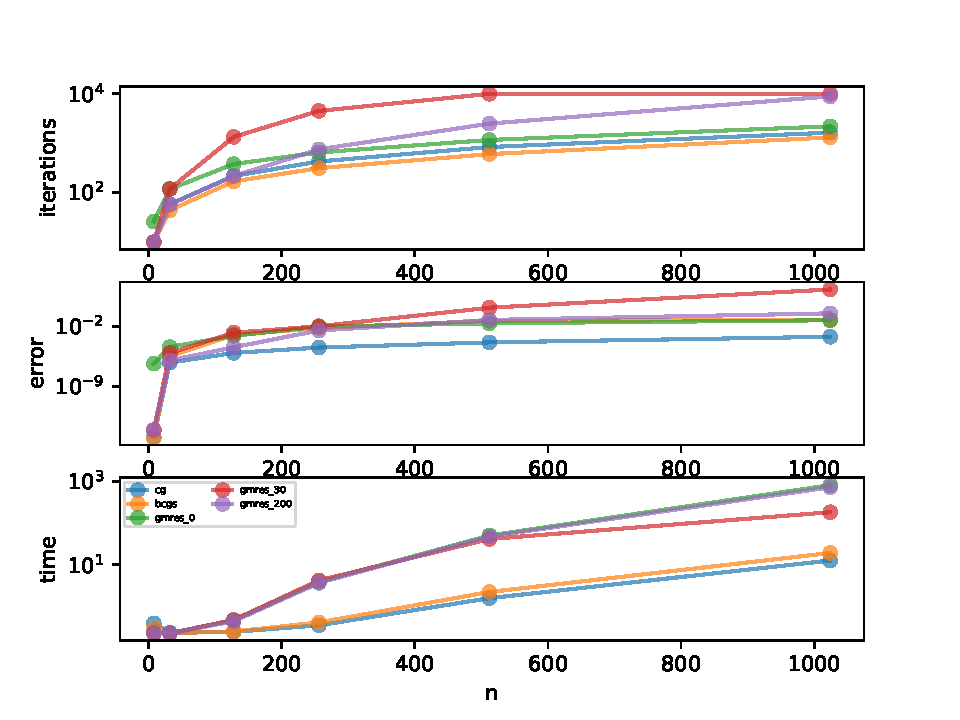
\includegraphics[width=0.6\textwidth,trim={0 0 0 0cm},clip]{results_nocondition.pdf}
  % \vspace{-8pt}
  \caption{Curves of scaling of statistics of Krylov methods for various matrix sizes for \program. The GMRES methods have either no restart (iterating up to $n=m$ iterations), or restart at 30 or 200 iterations.}
  \label{fig:Ex2}
\end{figure}

From these results, it is evident that there are tradeoffs between time of iterations, and total iterations and the resulting error norm of the residual. The method that scales best with grid size is, in terms of runtime, is possibly the CG or BiCGSTAB methods, that require no restarts and take less time and less iterations.

When GMRES is run with restarts $r$ of 30 and 200 iterations, for small matricies of size $n<r$, the number of iterations does not change drastically, as the Krylov subspace is built up within $n$ iterations. However for larger matrices where $n>r$, the number of total iterations increases drastically, and even reaches the 10,000 iteration threshold tolerance for the largest matrices. This is due to the iterations restarting many times before building up the Krylov subspace to dimension $n$.


\section{Preconditioners}

The following results of the Krylov statistics for \program are shown in Table \ref{tab:Ex3a} and Figure \ref{fig:Ex3ab}. It should be noted that th GMRES methods have no restart, iterating up to $n=m$ iterations, and the ILU and ICC preconditioners are unable to be parallalized in \exe, and so \textit{mpiexec} was not used for runtimes.

\subsection{GMRS}
\begin{table}[htb!]
    \centering
    \caption{Summary of scaling of statistics of GMRES method preconditoners for various matrix sizes for \program. The GMRES methods have no restart (iterating up to $n=m$ iterations).}
    \label{tab:Ex3a_gmres}
    \begin{tabular}{|c|c|c|c|c|c|c|} \hline
        Matrix Size & None & Jacobi & SOR & ILU & ICC & GAMG \\ \hline
        8     &     26(0.248)   &      26(0.253)  &    17(0.253)  &    10(0.231)   &   10(0.231)   &    7(0.251)  \\ \hline
        32    &     118(0.256)   &      118(0.254)  &    42(0.247) &    27(0.233)   &   27(0.234)   &    7(0.257) \\ \hline
        128   &     379(0.672)   &     379(0.676)   &   117(0.394)   &   85(0.361)    &  85(0.362)    &   8(0.301) \\ \hline
        256   &     652(5.424)   &      652(5.425)  &    189(1.560)  &    142(1.499)   &   142(1.572)   &    9(0.446) \\ \hline
        512   &    1164(65.640)   &     1164(72.788)  &   327(14.323)  &   247(15.052)   &  247(15.635)   &    9(1.139) \\ \hline
        1024  &  2195(1289.856)   &   2195(1112.954)  &  630(176.528)  &  476(177.825)   & 476(188.280)   &    10(3.674) \\ \hline
    \end{tabular}
\end{table}

\begin{figure}[ht]
  \centering
  %  trim={<left> <lower> <right> <upper>}
  % \captionsetup{skip=-12pt,format=hang}
  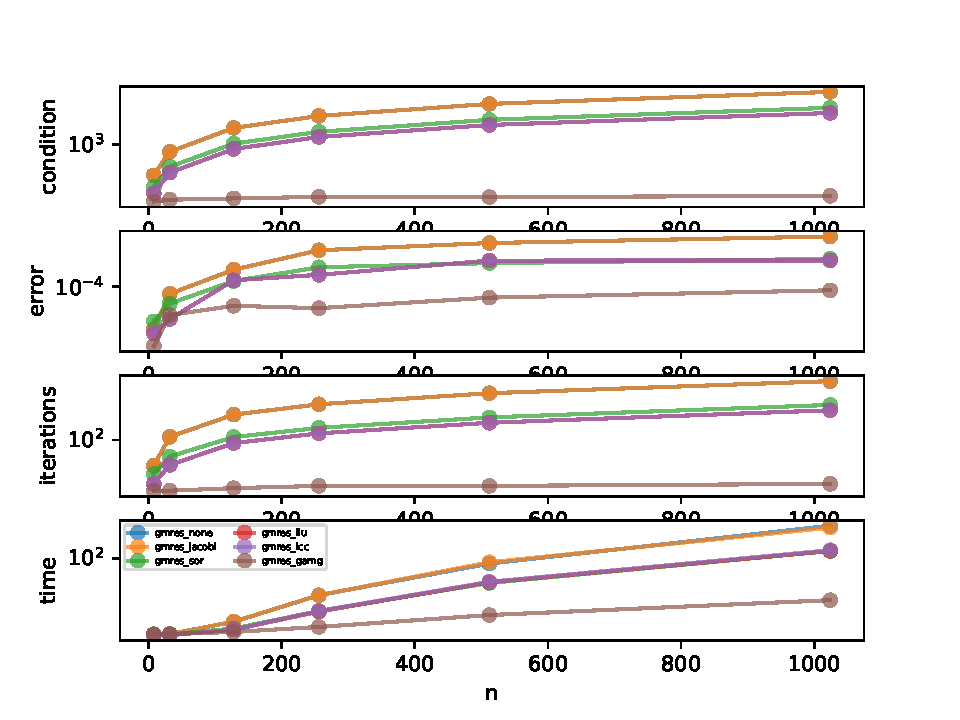
\includegraphics[width=0.6\textwidth,trim={0 0 0 0cm},clip]{results_gmres.pdf}
  % \vspace{-8pt}
  \caption{Curves of scaling of statistics of GMRES method preconditoners for various matrix sizes for \program. The GMRES methods have no restart (iterating up to $n=m$ iterations).}
  \label{fig:Ex3a_gmres}
\end{figure}

For the GMRES method, for time scaling, the preconditioners of \textit{none}, \textit{jacobi} and \textit{sor} all took similar time, and took longer much longer time than the \textit{ilu}, \textit{icc}, and \textit{gamg} methods. The time appears to obey approximately an exponential relationship with the size of the matrix.


For the GMRES method, the preconditioners that performed best, in terms of the \textit{gamg} algebraic multigrid method performed best, due to even at high matrix sizes, scaling the best. It used the least time and performed the least iterations, and still had the lowest residual error norm, and the lowest condition number estimate, compared to the other preconditioners.

When analysing the plots in \ref{fig:Ex3a_gmres} of run time and iterations versus matrix size, there is a direct, positive relationship between the scaling of the total runtime and number of iterations for each preconditioner. For each preconditioner, the total runtime appears to scale approximately exponentially with matrix size, and the number of iterations appears to scale polynomially with matrix size. The order of the preconditioners, in terms of slowest to fasest methods appears to be the same when looking at total runtime or number of iterations, with the \textit{gamg} being fastest, then \textit{ilu} and \textit{icc}, and then \textit{none} \textit{jacobi}, and \textit{sor} methods being slowest.


\subsection{CG}
\begin{table}[htb!]
    \centering
    \caption{Summary of scaling of statistics of CG method preconditoners for various matrix sizes for \program.}
    \label{tab:Ex3a_cg}
    \begin{tabular}{|c|c|c|c|c|c|c|} \hline
        Matrix Size & None & Jacobi & SOR & ILU & ICC & GAMG \\ \hline
        8   &    10(0.798)  &    10(0.236) &  15(0.237) &  9(0.228) &  9(0.226)  &  7(0.355) \\ \hline
        32  &    58(0.240)  &    58(0.241) &  42(0.239) &  9(0.223) &  27(0.227)  &  8(0.242) \\ \hline
        128 &    218(0.451)  &    218(0.446) &  122(0.312) &  27(0.278) &  88(0.277)  &  9(0.285) \\ \hline
        256 &    427(1.588)  &    427(1.595) &  204(0.572) &  88(0.502) &  145(0.489)  &  9(0.420) \\ \hline
        512 &   838(10.190)  &   838(10.166) &  336(2.202) &  145(2.071) &  277(2.084)  &  10(1.035) \\ \hline
        1024 &   1637(73.899)  &   1637(73.554) &  651(17.286) &  277(13.455) & 489(13.844) &  11(4.030) \\ \hline
    \end{tabular}
\end{table}

\begin{figure}[ht]
  \centering
  %  trim={<left> <lower> <right> <upper>}
  % \captionsetup{skip=-12pt,format=hang}
  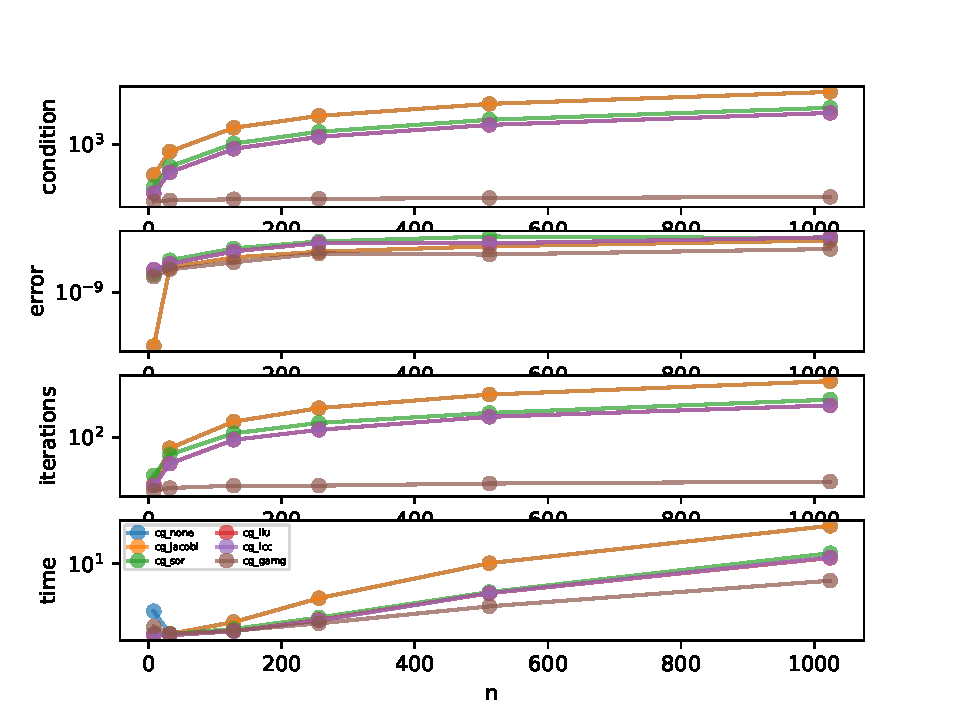
\includegraphics[width=0.6\textwidth,trim={0 0 0 0cm},clip]{results_cg.pdf}
  % \vspace{-8pt}
  \caption{Curves of scaling of statistics of CG method preconditoners for various matrix sizes for \program.}
  \label{fig:Ex3a_cg}
\end{figure}

For each preconditioner, the options are as follows, for example \cmd{time mpiexec -n 2 ./ex15 -ksp\_type gmres -n 1024 -m 1024 -pc\_type jacobi} \cmd{-ksp\_monitor\_singular\_value  -ksp\_gmres\_restart 1024}
where the \textit{pc\_type} passes in the preconditioner type.



\section{GMRES Error Scaling and Condition Number}

For each preconditioner, the options are as follows, for example \cmd{time mpiexec -n 2 ./ex15 -ksp\_type gmres -n 1024 -m 1024 -pc\_type jacobi} \cmd{-ksp\_monitor\_singular\_value -ksp\_gmres\_restart 1024}
where the \textit{pc\_type} passes in the preconditioner type, and the \textit{ksp\_monitor\_singular\_value} allows the condition number to be estimated as the ratio of the approximated maximum and minimum singular values.

\begin{table}[htb!]
    \centering
    \caption{Summary of condition number estimates from GMRES method preconditoners for various matrix sizes for \program.}
    \label{tab:Ex3b_gmres}
    \begin{tabular}{|c|c|c|c|c|c|c|} \hline
        Matrix Size & None & Jacobi & SOR & ILU & ICC & GAMG \\ \hline
        8   &   28.8956    &  28.8956 &  7.53438  & 3.58455  & 3.58455  &  1.42788 \\ \hline
        32  &    433.996   &  433.996 &  77.4939  & 39.6772 &  39.6772  &  1.74397 \\ \hline
        128 &    6729.31   &  6729.31  &  1100.5  & 596.623  & 596.623  &  2.02631 \\ \hline
        256 &    26733.1   &   26733.1 &  4315.74 &  2366.39  & 2366.39 &   2.40286 \\ \hline
        512 &   106549     &  106549  & 17099.2  & 9427.55 &  9427.55  &  2.35848 \\ \hline
        1024 &   425414    &   425414 &  68075.4 &  37636.1  & 37636.1 &   2.72101 \\ \hline
    \end{tabular}
\end{table}


When looking at the condition numbers using the preconditioners, the most efficient reduction in condition number was algebraic multigrid \textit{gamg} method, which is orders of magnitude lower than the other methods, and original condition number. This also directly corresponds to the number of iterations required, and the time taken to complete the algorithm, with this algebraic multigrid method being signicifantly faster than the other methods.


\section{CG Error Scaling and Condition Number}

For each preconditioner, the options are as follows, for example \cmd{time mpiexec -n 2 ./ex15 -ksp\_type cg -n 1024 -m 1024 -pc\_type jacobi} \cmd{-ksp\_monitor\_singular\_value}
where the \textit{pc\_type} passes in the preconditioner type, and the \textit{ksp\_monitor\_singular\_value} allows the condition number to be estimated as the ratio of the approximated maximum and minimum singular values.


\begin{table}[htb!]
    \centering
    \caption{Summary of condition number estimates from CG method preconditoners for various matrix sizes for \program.}
    \label{tab:Ex3b_cg}
    \begin{tabular}{|c|c|c|c|c|c|c|} \hline
        Matrix Size & None & Jacobi & SOR & ILU & ICC & GAMG \\ \hline
        8   &   29.2841  & 29.2841 & 7.66582 & 3.60845 & 3.60845 & 1.38219 \\ \hline
        32  &    437.698  & 437.698 &  76.852 &  39.665 &  39.665 & 1.56475 \\ \hline
        128 &    6740.68  & 6740.68 & 1097.26 & 596.647 & 596.647 & 1.77385 \\ \hline
        256 &    26765    & 26765 & 4310.33 & 2366.41 & 2366.41 & 1.86193 \\ \hline
        512 &   106549   &    106549 &  17099.2 &  9427.55 &  9427.55 &   2.35848 \\ \hline
        1024 &   425799  &  425799 & 68050.5 & 37636.2 & 37636.2 & 2.31255 \\ \hline
    \end{tabular}
\end{table}


When looking at the condition number $\kappa$ of the bare congugate gradient method (without preconditioning), when viewed as a function of matrix size $n$, and viewing the residual error norm $e$ as a function of matrix size, these data can be used to find a bound on the error. As shown in Figure \ref{fig:Ex4}, the error is shown to be bounded at least by the equation
$$ e(n) \leq 2\left(\frac{\sqrt{\kappa(n)}-1}{\sqrt{\kappa(n)}+1}\right)^{k(n)}.$$


\begin{figure}[ht]
  \centering
  %  trim={<left> <lower> <right> <upper>}
  % \captionsetup{skip=-12pt,format=hang}
  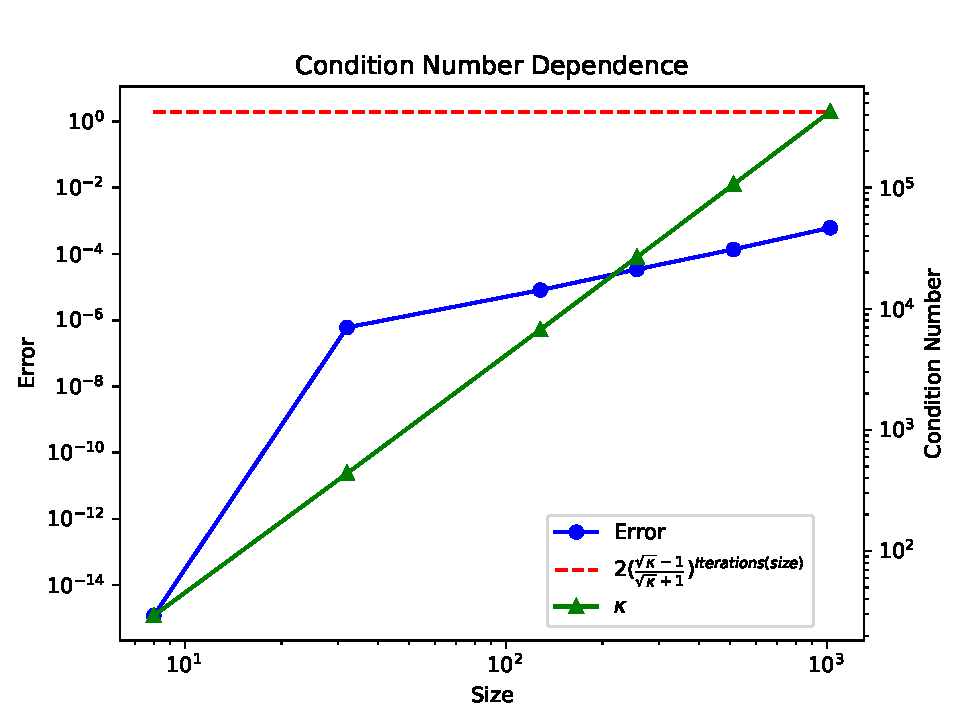
\includegraphics[width=0.6\textwidth,trim={0 0 0 0cm},clip]{results_fittedmodel.pdf}
  % \vspace{-8pt}
  \caption{Curves of scaling of error and condition number for the CG method as a function of matrix size, for \program.}
  \label{fig:Ex4}
\end{figure}



\newpage
\section{Appendix}

\subsection{\textit{install.sh}}
%\begin{verbatim}
\verbatiminput{FILES/install.sh}
%\end{verbatim}

\newpage
\subsection{\textit{run.py}}
%\begin{verbatim}
\verbatiminput{FILES/run.py}
%\end{verbatim}

\newpage
\subsection{\textit{job.slurm}}
%\begin{verbatim}
\verbatiminput{FILES/job.slurm}
%\end{verbatim}

\newpage
\subsection{\textit{process.sh}}
%\begin{verbatim}
\verbatiminput{FILES/process.sh}
%\end{verbatim}

\newpage
\subsection{\textit{plot.py}}
%\begin{verbatim}
\verbatiminput{FILES/plot.py}
%\end{verbatim}

\newpage
\subsection{\textit{run.sh}}
%\begin{verbatim}
\verbatiminput{FILES/run.sh}
%\end{verbatim}


%%%%%%%%%%%%%%%%%%%%%%%%%%%%%%%%%%%%%%%%%%%%%%%%%%%%%%%%%%%%%%%%%%%%%%%%%%%%%%%%%%%%%%%%%%%%%%%%%%%%%%%%%%%%%

% key condition
% 0       cg_none cg_jacobi   cg_sor   cg_ilu   cg_icc  cg_gamg
% size                                                         
% 8.0     29.2841   29.2841  7.66582  3.60845  3.60845  1.38219
% 32.0    437.698   437.698   76.852   39.665   39.665  1.56475
% 128.0   6740.68   6740.68  1097.26  596.647  596.647  1.77385
% 256.0     26765     26765  4310.33  2366.41  2366.41  1.86193
% 512.0    106655    106655  17088.1   9427.7   9427.7  2.04925
% 1024.0   425799    425799  68050.5  37636.2  37636.2  2.31255

% key error
% 0           cg_none    cg_jacobi       cg_sor       cg_ilu       cg_icc      cg_gamg
% size                                                                                
% 8.0     1.19575e-15  1.19575e-15  1.04748e-07  3.58257e-07  3.58257e-07  5.86979e-08
% 32.0    6.04802e-07  6.04802e-07  3.90533e-06  1.56076e-06  1.56076e-06   3.8421e-07
% 128.0    8.1102e-06   8.1102e-06     7.98e-05  3.81209e-05  3.81209e-05  2.30452e-06
% 256.0   3.43635e-05  3.43635e-05  0.000469078  0.000314674  0.000314674   2.2204e-05
% 512.0   0.000138048  0.000138048   0.00168338  0.000288775  0.000288775  1.69225e-05
% 1024.0  0.000619998  0.000619998   0.00109516   0.00138557   0.00138557  6.88555e-05

% key iterations
% 0    cg_none cg_jacobi cg_sor cg_ilu cg_icc cg_gamg
% size                                               
% 8         10        10     15      9      9       7
% 32        58        58     42     27     27       8
% 128      218       218    122     88     88       9
% 256      427       427    204    145    145       9
% 512      838       838    336    277    277      10
% 1024    1637      1637    651    489    489      11

% key time
% 0     cg_none  cg_jacobi  cg_sor  cg_ilu  cg_icc  cg_gamg
% size                                                     
% 8       0.798      0.236   0.237   0.228   0.226    0.355
% 32      0.240      0.241   0.239   0.223   0.227    0.242
% 128     0.451      0.446   0.312   0.278   0.277    0.285
% 256     1.588      1.595   0.572   0.502   0.489    0.420
% 512    10.190     10.166   2.202   2.071   2.084    1.035
% 1024   73.899     73.554  17.286  13.455  13.844    4.030

% key condition
% 0      gmres_none gmres_jacobi gmres_sor gmres_ilu gmres_icc gmres_gamg
% size                                                                   
% 8.0       28.8956      28.8956   7.53438   3.58455   3.58455    1.42788
% 32.0      433.996      433.996   77.4939   39.6772   39.6772    1.74397
% 128.0     6729.31      6729.31    1100.5   596.623   596.623    2.02631
% 256.0     26733.1      26733.1   4315.74   2366.39   2366.39    2.40286
% 512.0      106549       106549   17099.2   9427.55   9427.55    2.35848
% 1024.0     425414       425414   68075.4   37636.1   37636.1    2.72101

% key error
% 0        gmres_none gmres_jacobi    gmres_sor    gmres_ilu    gmres_icc   gmres_gamg
% size                                                                                
% 8.0     4.58704e-07  4.58704e-07  1.24654e-06  2.74612e-07  2.74612e-07   5.6142e-08
% 32.0    3.96713e-05  3.96713e-05  1.16629e-05  1.67065e-06  1.67065e-06  2.78486e-06
% 128.0   0.000816721  0.000816721  0.000197288  0.000217389  0.000217389  8.78212e-06
% 256.0    0.00940311   0.00940311   0.00110935  0.000429111  0.000429111  6.54164e-06
% 512.0     0.0232598    0.0232598   0.00187008   0.00257167   0.00257167  2.45119e-05
% 1024.0    0.0528249    0.0528249   0.00318741   0.00261812   0.00261812  6.16166e-05

% key iterations
% 0    gmres_none gmres_jacobi gmres_sor gmres_ilu gmres_icc gmres_gamg
% size                                                                 
% 8            26           26        17        10        10          7
% 32          118          118        42        27        27          7
% 128         379          379       117        85        85          8
% 256         652          652       189       142       142          9
% 512        1164         1164       327       247       247          9
% 1024       2195         2195       630       476       476         10

% key time
% 0     gmres_none  gmres_jacobi  gmres_sor  gmres_ilu  gmres_icc  gmres_gamg
% size                                                                       
% 8          0.248         0.253      0.253      0.231      0.231       0.251
% 32         0.256         0.254      0.247      0.233      0.234       0.257
% 128        0.672         0.676      0.394      0.361      0.362       0.301
% 256        5.424         5.425      1.560      1.499      1.572       0.446
% 512       65.640        72.788     14.323     15.052     15.635       1.139
% 1024    1289.856      1112.954    176.528    177.825    188.280       3.674









%%%%%%%%%%%%%%%%%%%%%%%%%%%%%%%%%%%%%%%%%%%%%%%%
% \newpage
% \bibliographystyle{unsrt}
% \bibliography{mduschen_Ex1.bib}

\end{document}